\chapter{Einleitung}
\section{Was ist Statistik?}
Im alltäglichen Sprachgebrauch versteht man unter \emph{Statistik} die
Auswertung und Darstellung von Daten und Fakten jeglicher Art. Diese Daten
können z.B. ökonomische Kenngrößen, Ergebnisse politischer Umfragen, Daten der
Marktforschung oder Ergebnisse klinischer Studien in der Medizin sein.

Die mathematische Statistik jedoch ist ein Teilgebiet der Stochastik und
entwickelt Regeln und Verfahren für die Erhebung, Beschreibung, Analyse und
Interpretation von Daten. Sie arbeitet mit Daten-Stichproben, die nach einem
bestimmten Zufallsmechanismus aus der Grundgesamtheit aller Daten gewonnen
werden. Die Daten wurden dabei in Folge von Beobachtung, Experimenten (reale
Daten) oder Computersimulation (synthetische Daten) erhoben. Dabei beschäftigt
sich die mathematische Statistik mit folgenden Fragestellungen:
\begin{enumerate}
\item Wie sollen die Daten gewonnen werden?
  $\rightarrow$ (Statistische Versuchsplanung)
\item  Wie lassen sich Datensätze beschreiben, grafisch aufarbeiten oder
  komprimieren, um eventuelle Gesetzmäßigkeiten und Strukturen in ihnen
  entdecken zu können? \\
  $\rightarrow$ (Beschreibende oder deskriptive Statistik)
\item Wie lassen sich die Daten analysieren und interpretieren? \\
  $\rightarrow$ (Schließende oder induktive Statistik)
\end{enumerate}

\begin{center}
  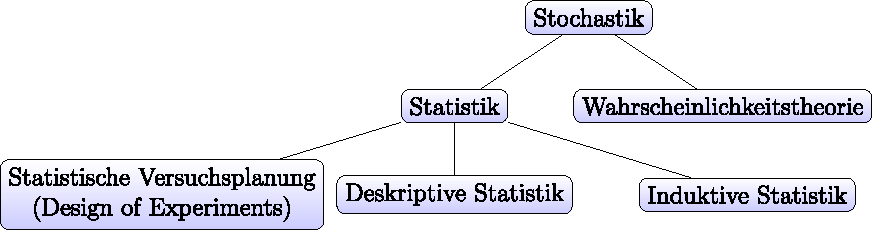
\includegraphics{img/stat_gruppen}
\end{center}

In dieser Vorlesung werden wir uns nur mit der deskriptiven und induktiven
Statistik befassen und die Versuchsplanung außer acht lassen.
Der typische Arbeitsverlauf eines Statistikers sieht etwa folgendermaßen aus:
\begin{enumerate}
\item Versuchsplanung und Datenerhebung
\item Visualisierung der Daten und deskriptive Datenanalyse
\item Datenbereinigung (z.B. Erkennung fehlerhafter Messungen, Ausreißern, usw.)
\item Explorative Datenanalyse (Suche nach Gesetzmäßigkeiten)
\item Modellierung der Daten mit Methoden der Stochastik
\item Modellanpassung (Schätzung der Modellparameter)
\item Modellvalidierung (wie gut war die Modellanpassung?)
\item Induktive Datenanalyse:
  \begin{enumerate}[(i)]
  \item Tests statistischer Hypothesen
  \item Konstruktion von Vertrauensintervallen (Konfidenzintervallen) für
    Modellparameter und deren Funktionen
  \item Vorhersage von Zielgrößen (z.B. auf Basis modellbezogener
    Computersimulation).
  \end{enumerate}
\end{enumerate}

Im Folgenden betrachten wir ein paar Beispiele für statistische Fragestellungen.

\begin{exmp}[Sonntagsfrage] ”Wenn am nächsten Sonntag Bundestagswahl wäre...”,
  mit dieser Frage, an jeweils etwa 2500 zufällig ausgewählte Wahlberechtigte
  gestellt, versucht die Forsa allwöchentlich Prognosen für den Ausgang einer
  (eventuell) bevorstehenden Bundestagswahl zu ermitteln. Neben dem konkreten
  Abschneiden der Parteien interessieren hier auch zeitliche Trends von Woche zu
  Woche.
\end{exmp}

\begin{exmp}[Wetteraufzeichnung]
  Durch kontinuierliches Sammeln und Auswerten von Wetterdaten wie z.B.
  Temperatur und Niederschlagsmenge, Windstärke (Beaufortskala, 0 bis 12),
  Bewölkung (heiter, heiter bis wolkig, wolkig), wird versucht, bessere
  Prognosen (Wettervorhersagen) zu erreichen und Trends (Klimaveränderungen) zu
  erkennen. Da Wetterdaten nur für ausgewählte Standorte zur Verfügung stehen,
  gehört zur Wettervorsage auch immer eine räumliche Interpolation.
\end{exmp}

\section{Grundbegriffe der Statistik}
Wir führen zunächst einige statistische Grundbegriffe ein:

\begin{tabular}{r|l}
  Statistische Einheit & Objekt, an dem interessierende Größen erfasst werden \\
  \\
  Grundgesamtheit / &  Menge aller relevanten statistischen Einheiten \\
  Population \\
  \\
  Teilgesamtheit & Teilmenge der Grundgesamtheit \\
  \\
  Stichprobe & untersuchte Teilmenge der Grundgesamtheit \\
  \\
  Merkmal/Variable & interessierende Größe \\
  \\
  Merkmalsausprägung/-wert & konkreter Wert eines Merkmals für eine
                             konkrete Einheit
\end{tabular}

Die Population bezeichnen wir mit $\Omega$, eine einzelne Einheit mit $\omega
\in \Omega$. Die Merkmalsausprägung der Einheit $\omega$ notieren wir mit
$X(\omega)$.

Beachte:
\begin{itemize}
\item $X(\omega)$ kann als Zufallsvariable aufgefasst werden.
\item Die Grundgesamtheit $\Omega$ kann auch überabzählbar sein.
\item In der Praxis liegt die Grundgesamtheit oft nur \emph{hypothetisch} vor,
  z.B. wenn eine KfZ-Versicherung das Fahrverhalten aller \emph{potenziellen}
  Kunden modellieren will.
\end{itemize}

\begin{exmp}
  Bei der Sonntagsfrage (Beispiel 1.1) ist die Grundgesamtheit die Menge aller
  wahlberechtigten Bürger Deutschlands. Eine mögliche Teilgesamtheit wären z.B.
  alle Erstwähler. Stichprobe sind die zu dem jeweiligen Sonntag befragten
  Bürger. Das statistische Merkmal jeder Einheit ist die gewählte Partei,
  mögliche Ausprägungen sind also z.B. CDU, SPD, Grüne, Linke, ...
\end{exmp}

\begin{exmp}[DAX30]
  In Tabelle 1.4 sind die jährlichen Renditen (Merkmale ”re2005” bis ”re2010”)
  der 30 DAX Unternehmen (Einheiten) für die Jahre 2005 bis 2010 angegeben.
  Zudem sind als weitere Merkmale für jedes Unternehmen der Unternehmensname
  (”company”) und die zugehörige Branche aufgeführt, wobei zwei
  Kategorisierungen verwendet werden: Das Merkmal ”sector” besitzt die 9
  Ausprägungen ”automobile”, ”chemical”, ”financial”, ”health”, ”industrial”,
  ”IT”, ”retail”, ”transport” und ”utilities”, während das übergeordnete Merkmal
  ”zone” lediglich die 6 Ausprägungen ”automobile”, ”chem.health”, ”financial”,
  ”industrial”, ”retail” und ”trans.util.it” besitzt.
  
  Als Grundgesamtheit kann hier z.B. die Menge aller börsennotierten Unternehmen
  in Deutschland angenommen werden, Stichprobe sind die 30 DAX-Unternehmen.
  
  Die Daten stehen auch als Datei ”dax30.dat” auf der Vorlesungswebseite zur
  Verfügung und können folgendermaßen in R eingelesen werden:
  \begin{verbatim}
#Daten einlesen:
dax<-read.table(file="dax30.dat",header=T)
#Daten als Tabelle ausgeben:
dax
  \end{verbatim}
\end{exmp}

In der deskriptiven Statistik visualisiert man Stichproben/Daten $(x_1, \ldots,
x_n)$ und Funktionen dieser Daten. Für die Aufgabe der induktiven Statistik
jedoch reicht diese Datenebene nicht mehr aus. Daher wird die zweite Ebene der
Betrachtung eingeführt, die sogenannte Modellebene. Dabei wird angenommen,
dass die konkrete Stichprobe $(x_1, \ldots, x_n)$ eine Realisierung eines
stochastischen Modells $(X_1, \ldots, X_n)$ darstellt, wobei $X_1, \ldots,
X_n$ (meistens unabhängige, identisch verteilte) Zufallsvariablen auf einem
(meist nicht näher spezifizierten) Wahrscheinlichkeitsraum $(\omega, F, \pP)$
sind. Die Zufallsvariablen $X_i$ werden dann als Beobachtungen eines Merkmals
interpretiert und der Vektor $(X_1, \ldots, X_n)$ als Zufallsstichprobe
bezeichnet.
  
Eine zentrale Fragestellung der Statistik ist das Bestimmen der
Verteilungsfunktion $F$ (Schätzung von $F$) der Zufallsvariablen $X_i$ aus den
konkreten Daten $(x_1, \ldots, x_n)$. Dabei können neben der eigentlichen
Funktion $F$ z.B. auch Momente von $F$ und ihre Funktionen (Erwartungswert,
Varianz, Schiefe, usw.) von Interesse sein.

Um diese Aufgaben zu lösen, werden sogenannte Stichprobenfunktionen $\phi :
\real^n \to \real^m$ definiert, d.h. Borel-messbare Funktionen, welche die
gegebene Stichprobe bewerten. Auf der Modellebene angewandt, wird die
Zufallsvariable
\[ \phi(X_1, \ldots, X_n) \]
als Statistik bezeichnet. In der Schätztheorie (siehe Kapitel 3) spricht man
stattdessen auch von einem Schätzer und bei statistischen Tests (siehe Kapitel
4) von einer Teststatistik.

Beispiele für Stichprobenfunktionen sind unter anderen
\begin{itemize}
\item empirischer Erwartungswert/Stichprobenmittel/arithmetisches Mittel
  \[ \obar{x} = \rez{n} \sum_{i=1}^n x_i, \]
  (nur für Daten anwendbar, welche als Zahlenwerte vorliegen),
\item empirische Varianz/Stichprobenvarianz
  \[s^2 = \rez{n-1} \sum_{i=1}^n (x - \bar{x})^2 \]
  (nur für Daten anwendbar, welche als Zahlenwerte vorliegen),
\item die Ordnungsstatistik von $x_1, \ldots, x_n$, welche entsteht, indem man
  die Stichprobe aufsteigend ordnet (nur für Daten anwendbar, die einer Ordnng
  unterliegen).
\end{itemize}

\section{Statistische Merkmale}
Wie aus den obigen Beispielen ersichtlich ist, können statistische Merkmale von
ganz unterschiedlicher Natur sein. Um später sinnvoll mit erhobenen Daten
arbeiten zu können, werden die Merkmale daher nach Eigenschaften ihrer
Ausprägungen klassifiziert. Wir unterscheiden zunächst zwischen stetigen und
diskreten Merkmalen:

\begin{center}
  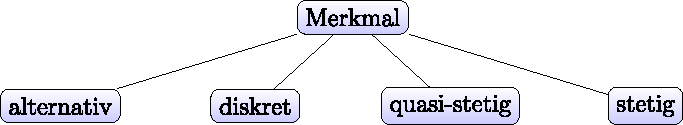
\includegraphics{img/merkmale_stetig_diskret}
\end{center}

Hierbei gelten:
\begin{center}
  \begin{tabular}{r|p{12cm}}
    alternativ & Merkmal besitzt genau zwei Ausprägungen \\
    \\
    diskret & Merkmal kann nur endlich viele verschiedene Werte annehmen \\
    \\
    stetig & kann alle Werte innerhalb eines Intervalls annehmen \\
    \\
    quasi-stetig & nur diskret messbar, allerdings mit sehr feiner Abstufung,
                   so dass das Merkmal wie ein stetiges Merkmal behandelt
                   werden kann.
  \end{tabular}
\end{center}

Zudem unterscheiden wir die folgenden Merkmalstypen und Merkmalsskalen:

\begin{center}
  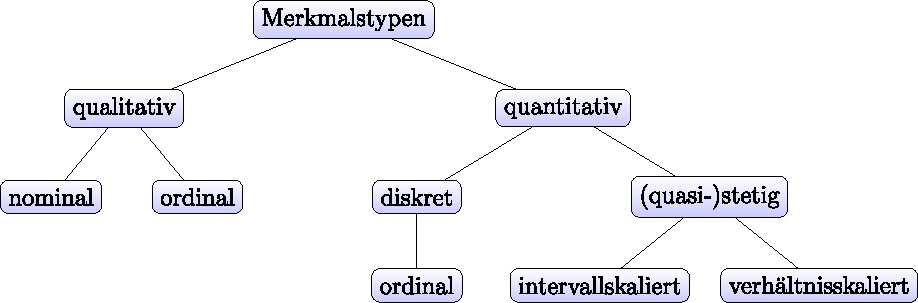
\includegraphics{img/merkmalstypen}
\end{center}

\begin{center}
  \begin{tabular}{r|p{12cm}}
    qualitativ/kategorial & keine inhaltlich sinnvolle Darstellung durch
                            Zahlenwerte möglich \\
    \\
    quantitativ & lässt sich inhaltlich sinnvoll durch Zahlenwerte
                  darstellen. \\
    \\
    nominal(skaliert) & Ausprägungen unterliegen keiner Ordnung \\
    \\
    ordinal(skaliert) & Ausprägungen können geordnet werden, Abstände
                        sind jedoch nicht notwendig interpretierbar \\
    \\
    intervallskaliert & Ausprägungen sind Zahlen, aber ohne absoluten
                        Nullpunkt \\
    \\
    verhältnisskaliert & Ausprägungen sind intervallskaliert und haben einen
                         absoluten Nullpunkt
  \end{tabular}
\end{center}

Beachte: Merkmalstypen und Skalen sind nicht immer eindeutig zuzuordnen:
\begin{itemize}
\item Jedes stetige Merkmal lässt sich durch Klassenbildung/gruppieren als
  diskretes Merkmal auffassen. Andererseits werden durch Abrunden in der Praxis
  keine (echt) stetigen Merkmale vorkommen.
\item Die obige Baumstruktur muss nicht unbedingt eingehalten werden. In
  gewissem Sinne (und in manchen Quellen) ist auch jedes quantitative Merkmal
  ordinalskaliert.
\item Beispiel Schulnoten: Diese können ordinal quantitativ aufgefasst werden
  (1, 2, 3, 4, 5, 6), oder alternativ ordinal qualitativ (sehr gut, gut,
  befriedigend,...). 
\item Häufig werden qualitative Merkmale für die Datenverarbeitung quantitativ
  kodiert. Durchschnittswerte sind dann unsinnig.
\end{itemize}

\begin{exmp}
  Bei der Sonntagsfrage (Beispiel 1.1) ist das Merkmal (die gewählte
  Partei) diskret, qualitativ und nominal.
  
  In der Wetteraufzeichnung (Beispiel 1.2) sind die Merkmale Temperatur und
  Niederschlagsmenge quantitativ und (quasi-)stetig. Die Temperatur
  ($\si{\celsius}$) ist intervallskaliert, während die
  Niederschlagsmenge verhältnisskaliert ist. Das Merkmal Windstärke ist
  quantitativ, diskret und verhältnisskaliert. Die Bewölkung ist ein diskretes,
  ordinales, qualitatives Merkmal.
\end{exmp}

Tabelle 1 siehe Skript.